\subsection{Funcionamento da turbina}
  
  O desenho esquemático da turbina apresentado na figura abaixo mostra as pás acopladas ao rotor, que por meio de um eixo cilíndrico conecta-se ao gerador. Este gerador é o responsável pela geração de energia elétrica através da energia mecânica. A energia mecânica é provinda do giro das hélices que os ventos provocam ao entrar em contato com as pás.  No compartimento à esquerda, onde se encontram o eixo do rotor e o gerador, contem também um filtro de partículas e dois cilindros de compressores. O filtro de partículas frontal é necessário para evitar que resíduos do ar danifiquem os componentes eletrônicos presentes nessa região, tendo em vista que há uma circulação de vento nesse compartimento com o âmbito de refrigerar o gerador e os compressores. Já os compressores, irão comprimir o gás presente em ductos (que estão acoplados ao condensador presente no outro compartimento) para que se atinja uma temperatura baixa possível de se realizar a condensação do ar.
  
  \FloatBarrier
  \begin{figure}[!h]
    \centering
    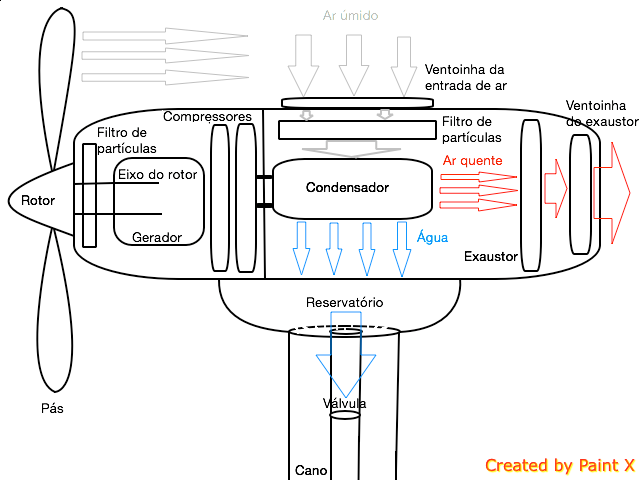
\includegraphics[scale = 0.9]{editaveis/figuras/funcionamento_turbina}
    \label{funcionamento_turbina}
    \caption[Funcionamento da turbina]{Desenho esquemático do funcionamento da turbina geradora de energia e água.}
  \end{figure}
  \FloatBarrier
    
  No segundo compartimento, que tem uma circulação de ventos independente do primeiro compartimento, estão presentes os componentes necessários para a captação de água através da umidade. A entrada de ar úmido se dá pelo topo da nacele por meio de uma ventoinha que suga o ar da atmosfera para dentro da turbina. Uma vez o ar úmido dentro da turbina, ele passa por um filtro de partículas para que as impurezas não danifiquem o funcionamento de nenhum componente. Filtrado o ar, este entra em contato com o condensador que, junto com os ductos vindos do compressor, irá condensar este ar. O ar condensado (líquido) escorre pelas paredes do condensador até cair no reservatório contido na base da nacele, enquanto o ar quente provocado pelo condensar neste processo é sugado por um exaustor e enviado diretamente para fora da nacele por meio de uma ventoinha presente no extremo oposto às pás. A água permanece no reservatório até que sensores permitam a abertura da válvula de escoamento que, uma vez aberta, toda a quantidade de líquido até então armazenada escorrerá, por ação da gravidade, pelo cano presente ao longo da torre de sustentação.
  O monitoramento do estado das turbinas será feito pelo sistema de gestão da informação com os dados obtidos pelos sensores na estrutura 
  da turbina.

\subsection{Monitoramento eletrônico e adição de sais}

  \begin{figure}[!htbp]
    \centering
    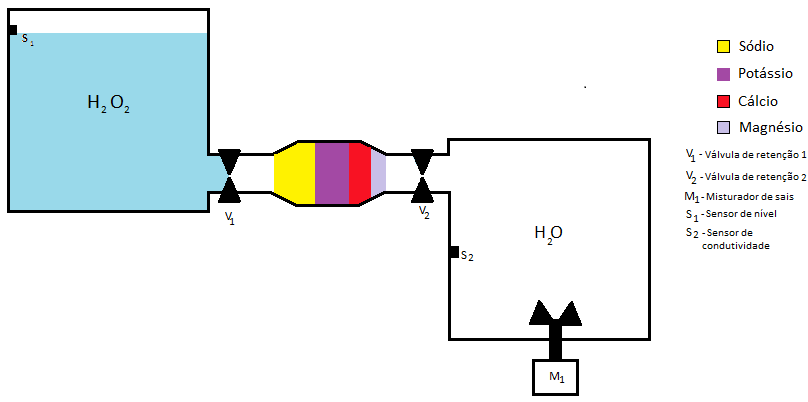
\includegraphics[scale=0.6]{editaveis/figuras/sistema_adicionador_sais}
    \caption[Esquemático do sistema adicionador de sais]{Esquemático do sistema adicionador de sais.}
    \label{sistema_adicionador_sais_1}
  \end{figure}
  \FloatBarrier
    
Após sair da turbina, a água irá descer pelo cano em direção ao reservatório. A água provinda da turbina contará com processos
mecânicos e digitais, sendo assim, após filtragem a água é direcionada para o tanque primário, o qual encherá até certo nível.
A água passará então por um filtro que adicionára os sais necessário à agua, jogando a àgua adicionada de sais em outro tanque,
onde há um misturador para realizar a solubilização dos sais na água.

Nestes reservatórios também se encontram os sensores necessários para o monitoramento da qualidade da água e dos níveis do reservatório.


\subsection{Monitoramento do sistema de gestão da informação}

  O controle de tais sensores se dará por meio do software, cuja finalidade principal é o monitoramento do sistema como um todo. Nele haverá informações relacionadas à qualidade e quantidade da água obtida, características do ambiente externo onde as turbinas se encontram casa de controle, distribuição de energia excedida, ao armazenamento e tratamento com sais da água ainda dados sobre a turbina.
	 
  Alguns dos dados referentes à turbina que serão monitorados pelo software são: as temperaturas internas, a quantidade de energia gerada por cada turbina, a velocidade de rotação das pás. A qualidade da água também será monitorada, pois o software fará as devidas leituras dos sensores, dados relacionados à casa de controle incluem, por exemplo, a voltagem das baterias, a falta ou presença de energia. Com relação à distribuição de energia, o software deve mostrar se a energia excedida está sendo direcionada a rede ou se está abastecendo a casa de controle.

  Também serão obtidos dados referentes à umidade do ar e as características do vento de onde as turbinas se encontram, como exemplo de dados relacionados ao ambiente externo. Percebe-se, portanto, que o software que será utilizado possibilitará o monitoramento de uma série de aspectos relacionados a tecnologia de captação de água a partir da umidade do ar.

  Além de realizar a manutenção da água, e os sensores que capacitam a boa qualidade da água distribuída, os softwares permitirão o cadastro de pessoas que chegarão para buscar a água. Isso permite que façamos um censo e adequemos o sistema a cada mudança de demanda por água, seja por que o número de pessoas atendidas tenha aumentado ou diminuído.

\subsection{Distribuição da água}
  A água será distribuída através de torneiras acopladas a parte externa da torre de controle, com acesso direto ao produto final. A água que ficar em excesso no reservatório será engarrafada em garrafas apropriadamente higienizadas, as quais serão cedidas pelas empresas parceiras. Sendo essas também responsáveis pelo destino das garrafas quando chegar a hora do descarte delas.
  
  \FloatBarrier
  \begin{figure}[!h]
      \centering
      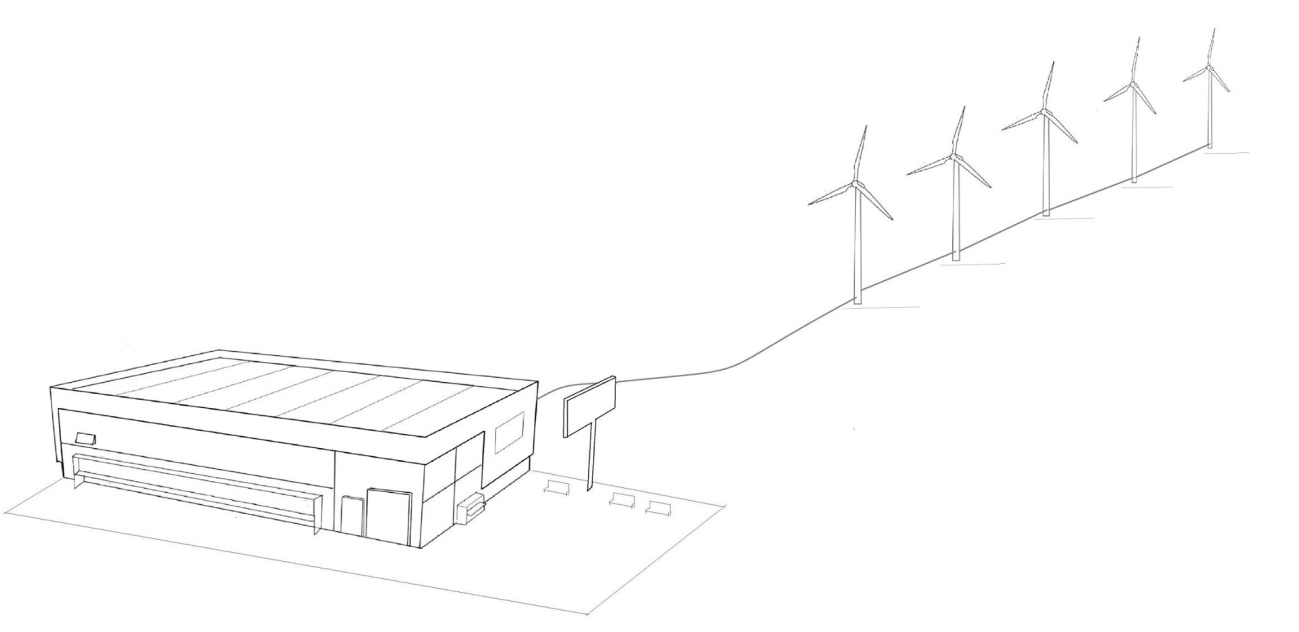
\includegraphics[scale = 0.4]{editaveis/figuras/distribuicao_agua}
      \label{distribuicao_agua}
      \caption[Distribuição água]{Esquema de distribuição da água até chegar ao local de distribuição.}
  \end{figure}
  \FloatBarrier
  
  A prefeitura Municipal de Acari, juntamente com empresas parceiras construirá uma praça de finalidade educacional da população, onde será localizado o centro de distribuição de água. A água será distribuída de forma gratuita, pois o projeto visa o lado social e a melhora na qualidade de vida.

